\documentclass[11pt, a4paper]{article}

\usepackage{graphicx}
\usepackage[a4paper,top=3cm,bottom=2cm,left=2cm,right=2cm,marginparwidth=1.75cm]{geometry}
\usepackage[english]{babel}
\usepackage[utf8x]{inputenc}
\usepackage{subfig}
\usepackage{float}
\usepackage{amsmath}
\usepackage{amssymb}
\usepackage{mhchem}
\usepackage{hyperref}
\usepackage{tikz}
\usepackage{cancel}
\usepackage{bm}

\graphicspath{ {./images} }
\newcommand*{\qed}{\hfill\ensuremath{\quad\square}}%
\newcommand*{\rad}{\ensuremath{\,\text{rad}}}
\newcommand*{\R}{\ensuremath{\mathbb{R}}}
\newcommand*{\C}{\ensuremath{\mathbb{C}}}
\renewcommand*{\Re}{\operatorname{Re}}
\renewcommand*{\Im}{\operatorname{Im}}
\renewcommand*{\epsilon}{\varepsilon}
\renewcommand*{\phi}{\varphi}
\renewcommand*{\d}{\text{d}}

\DeclareRobustCommand{\uvec}[1]{{%
  \ifcat\relax\noexpand#1%
    % it should be a Greek letter
    \bm{\hat{#1}}%
  \else
    \ifcsname uvec#1\endcsname
      \csname uvec#1\endcsname
    \else
      \bm{\hat{\mathbf{#1}}}%
     \fi
   \fi
}}

\makeatletter
\renewcommand*\env@matrix[1][*\c@MaxMatrixCols c]{%
  \hskip -\arraycolsep
  \let\@ifnextchar\new@ifnextchar
  \array{#1}}
\makeatother

\newtheorem{theorem}{Theorem}
\numberwithin{equation}{section}
\numberwithin{figure}{section}

%------------------------------------------------
%Templates for images and figures
% \begin{figure}[h]
%   \centering
%   \subfloat[caption 1]{{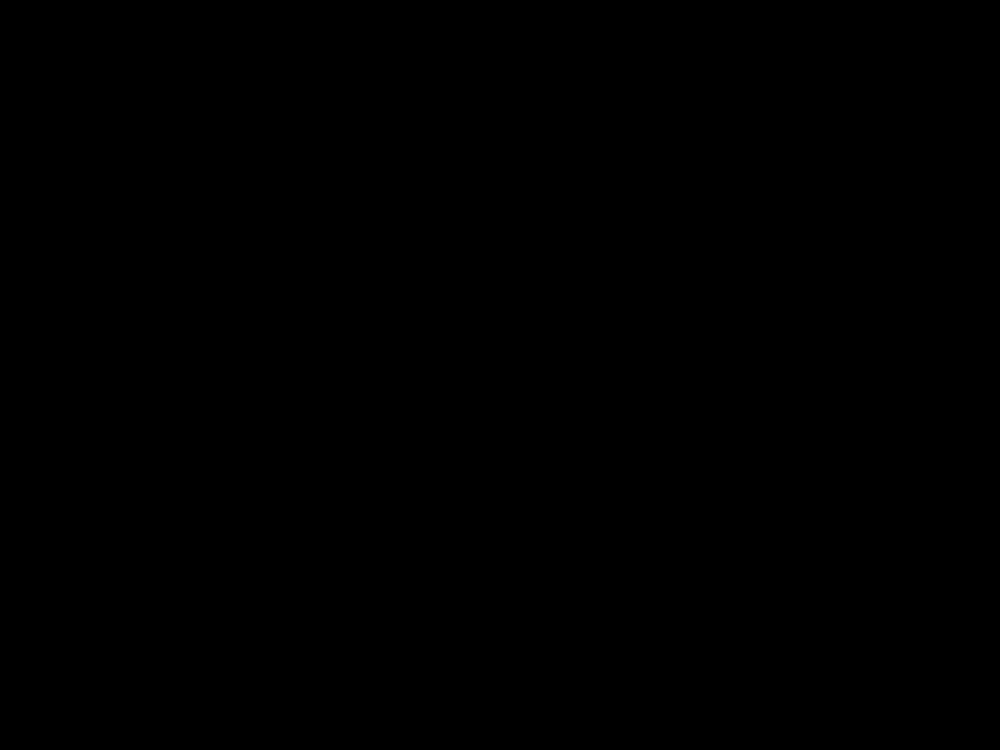
\includegraphics[width=30mm]{images/placeholder.png}}}%
%   \qquad
%   \subfloat[caption 2]{{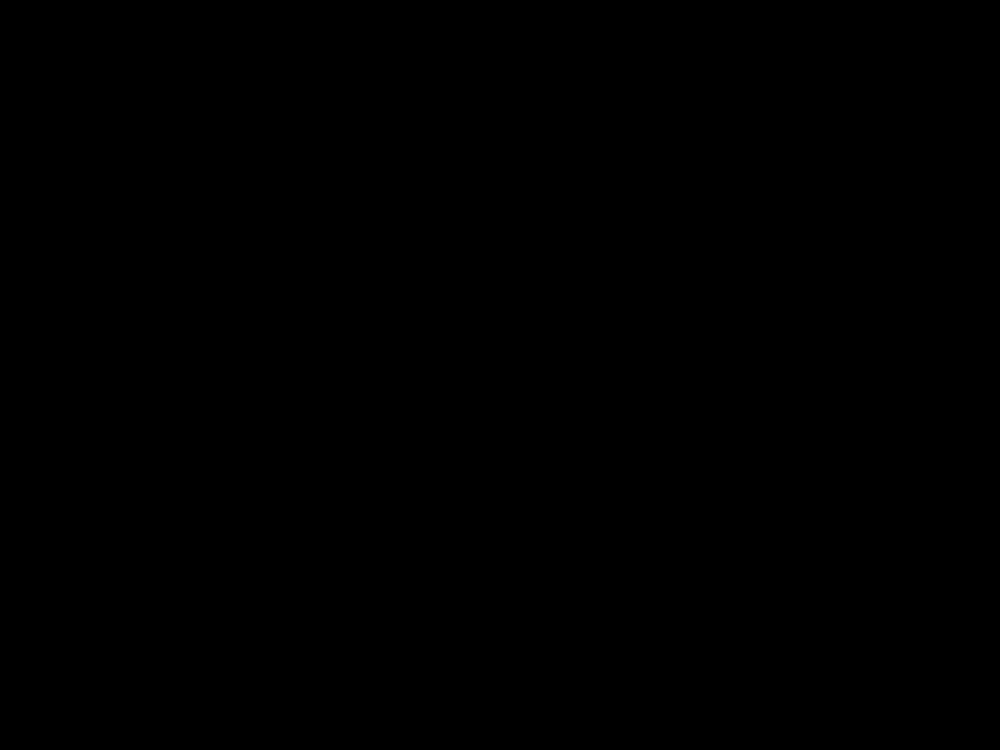
\includegraphics[width=30mm]{images/placeholder.png}}}%
%   \caption{Description}
% \end{figure}

% \begin{figure}[h]
%   \centerline{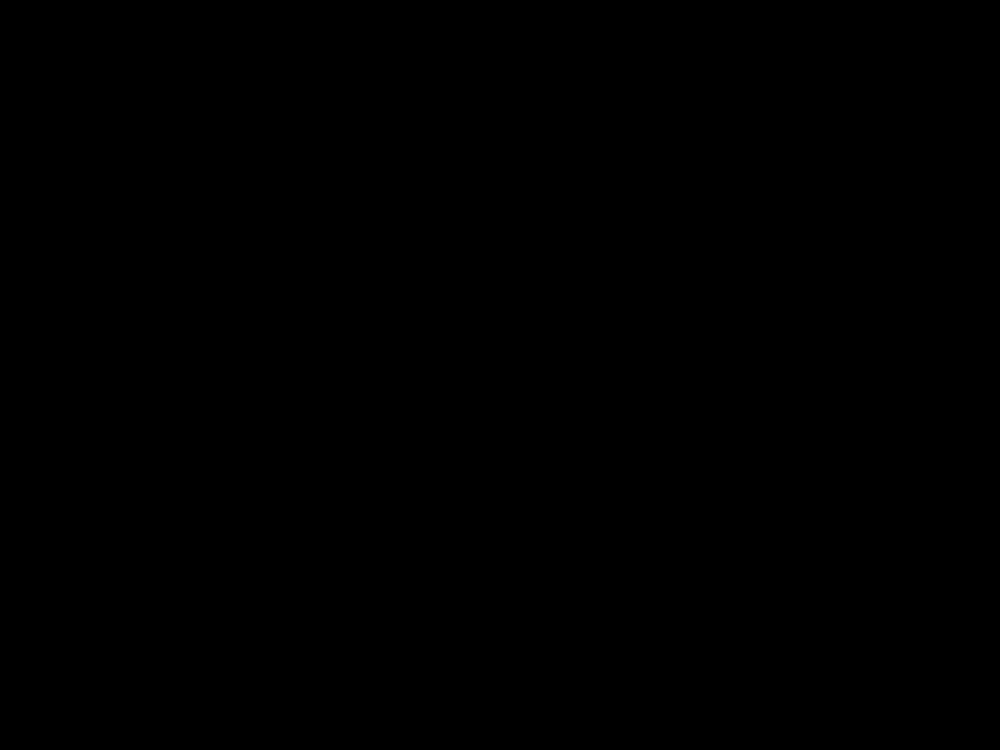
\includegraphics[width=50mm]{images/placeholder.png}}
%   \caption{Description}
% \end{figure}

%Template for a simple table 
%\begin{table}[h]
%   \caption{Description} %title of the table
%   \centering % centering table
%   \begin{tabular}{l rr} % creating three columns
%     \hline\hline %inserting double-line
%     & & \\ [0.5ex] % Insert half line vertical spacing
%     \hline % inserts single-line
%     & & \\ 
%     & & \\
%     & & \\
%     & & \\
%   \hline % inserts single-line
%   \end{tabular}
%   \label{tab:hresult}
% \end{table}
%-----------------------------------------------

\begin{document}
\setcounter{section}{5}
\section{Using potential energy}
\subsection{The spring system}
Consider the following spring system. When we would analyze this only using external virtual work we would end up with only 1 equation. We can include the equilibrium between internal and external work in our analysis to get 3 equations rather then 1 when analyzing this system. 
\begin{figure}[H]
  \centerline{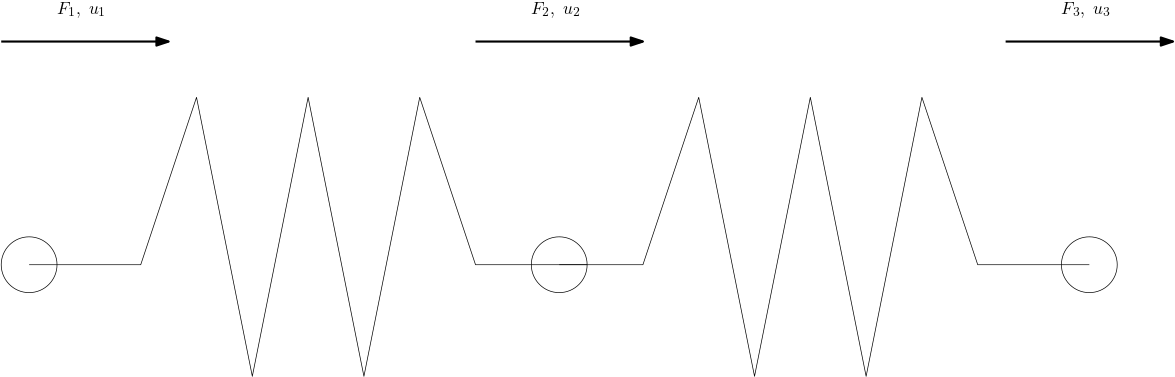
\includegraphics[width=100mm]{images/Springs.png}}
  \caption{The spring system being analyzed for internal and external balance of virtual work}
\end{figure}
We can easily see from the figure that:
\begin{gather}
  \Delta L_I = u_2 - u_1\\
  \Delta L_{II} = u_3 - u_2
\end{gather}
When considering an infinitesimal virtual displacement $\delta$ we get:
\begin{gather}
  \delta (\Delta L_I) = \delta u_2 - \delta u_1\\
  \delta (\Delta L_{II}) = \delta u_3 - \delta u_2
\end{gather}
From this we can derrive the following equation by substitution:
\begin{equation}
  \delta (\Delta L_I) = \frac{\partial \Delta L_I}{\partial u_1} \delta u_1 + \frac{\partial \Delta L_{II}}{\partial u_2} \delta u_2  
\end{equation}
We now consider the internal and external work of the system:
\begin{gather}
  \delta W_i = F_{v,I} \delta(\Delta L_I) + F_{v, II} \delta(\Delta L_{II})\\
  \delta W_u = F_1\delta u_1 + F_2\delta u_2 + F_3\delta u_3
\end{gather}
Applying the condition that $\delta W_i = \delta W_u$ since energy can not be created we can equate these to equations and find a system of 3 equations:
\begin{gather}
  F_{v,I}(\delta u_2 - \delta u_1) + F_{v,II}(\delta u_3 - \delta u_2) = F_1\delta u_1 + F_2 \delta u_2 + F_3 \delta u_3\\
  \begin{cases}
    F_1 = -F_{v,I}\\
    F_2 = F_{v,I} - F_{v, II}\\
    F_3 = F_{v,II}
  \end{cases}
\end{gather}
Thus we now derrived a system of 3 equations rather then 1 equation by also including internal virtual work in out equations.



\subsection{Minimum of potential energy}
Internal work is nothing but stored energy in the form of elasticity. This is a form of potential energy. The total potential of a system can be given by the following expression:
\begin{equation*}
  \mathcal{P}[\vec{u}_0] = \mathcal{E}[\vec{u}_0] + \mathcal{B}[\vec{u}_0]
\end{equation*}
Where $\mathcal{P}$ is the total potential, $\mathcal{E}$ the elastic potential and $\mathcal{B}$ the potential energy due to externally applied loads. $\vec{u}_0$ is a random displacement vector which is kinematically allowed. This means the displacement cannot break the continuity of the material. The following 2 additional relations exist:
\begin{align}
  \mathcal{P}[\vec{u}_0] &= \text{Stationary if there is equilibrium}\\
  \mathcal{P}[\vec{u}_0] &= \text{Local minimum if the equilibrium is stable}
\end{align}
There are 3 conditions which need to apply for analysis using potential energy to be valid.
\begin{enumerate}
  \item System must be elastic, though non-lineare behaviour is allowed
  \item No damping on the system
  \item System is conservative\footnote{This means that energy is conserved, not that the system supports right-wing politics}
\end{enumerate}
\begin{figure}[H]
  \centerline{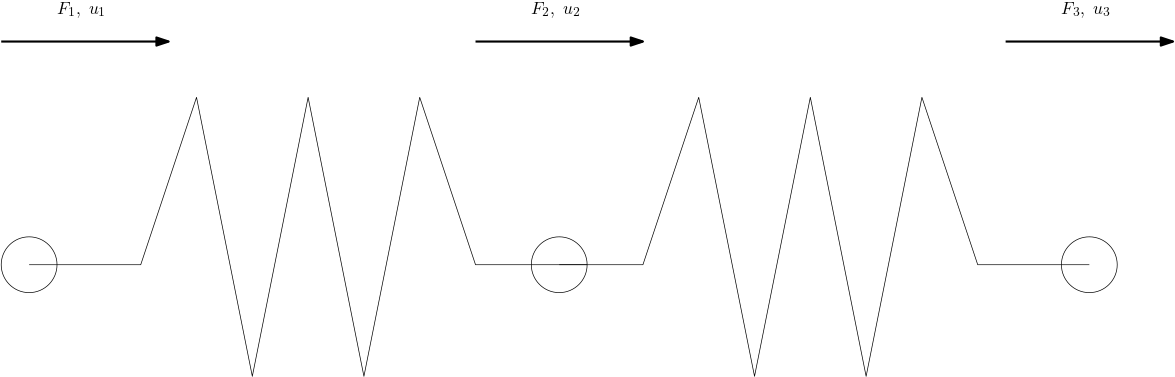
\includegraphics[width=100mm]{images/Springs.png}}
  \caption{Teh same spring system but this time applyign potential enrgy analysis}
\end{figure}
We can now again analyse the spring system, but this time using potential energy. We start again by defining displacements:
\begin{gather}
  \Delta L_I = u_2\\
  \Delta L_{II} = u_3 - u_2\\
\end{gather}
The elastic potential of this system is then given as:
\begin{equation}
  \mathcal{E} = \Sigma\mathcal{E}_i = \frac{1}{2}k u_2^2 + \frac{1}{2}k (u_3 - u_2)^2
\end{equation}
The load potential for this system is given as:
\begin{equation}
  \mathcal{B} = -F_3u_3
\end{equation}
Which is just the equilibrium condition. We can now derrive the total potential of the system.
\begin{equation}
  \mathcal{P} = \mathcal{E} + \mathcal{B} = \frac{1}{2}k u_2^2 + \frac{1}{2}k (u_3 - u_2)^2 - F_3u_3
\end{equation}
$\mathcal{P}$ must be a stationary value for equilibrium to exist. This implies that:
\begin{equation}
  \begin{cases}
    \frac{\partial \mathcal{P}}{\partial u_1} = 0\\
    \frac{\partial \mathcal{P}}{\partial u_2} = 0
  \end{cases}
\end{equation}
Thus for 2 variables we found a corresponding system of 2 equations.
\end{document}